\def\QRCODE{TB_image_TUT.IMG.segmentation_region_growing_pythonqrcode.png}
\def\QRPAGE{http://www.iptutorials.science/tree/master/TB_image/TUT.IMG.segmentation_region_growing/python}

\pcorrectionsection{Python correction}

\subsection{imports}

\begin{python}
import queue
from scipy import misc
import matplotlib.pyplot as plt
import numpy as np
\end{python}

\subsection{Predicate}
This function defines the agregation condition.
\begin{python}
def predicate(image, i, j, seed) :
	f=image[i,j];
	g=image[seed[0], seed[1]];
	return abs(f-g)<20
\end{python}
    
    
The following code is used to start the region growing from a pixel manually clicked on an image.
\begin{python}
# start of code
fig = plt.figure();
ax = fig.add_subplot(211);
ax.set_title('Click on a point')

# load image
img = misc.ascent();
ax.imshow(img, picker=True,cmap=plt.gray());

fig.canvas.mpl_connect('button_press_event', onpick)
plt.show();
\end{python}

And here comes the main function for region growing. The result is illustrated in Fig.\ref{fig:regiongrowing:python:result}.



\begin{python}
def onpick (event):
    """
    this functions gets the event 'click', and starts the region growing algorithm
    Notice that img is a global variable
    """
    print("x, y: ", event.xdata, event.ydata);
    # original pixel
    seed = np.array ([int (event.ydata), int (event.xdata)]);
    q = queue.Queue ();
    
    myfunctions = [predicate, predicate2, predicate3];

    for index,f in enumerate(myfunctions):     
        
        # initializes the queue
        q.put (seed);
   
        #Visited matrix : result of segmentation
        #this matrix will contain 1 if in the region, -1 if visited but not in the region, 0 if not visited
        visited = np.zeros (img.shape)
        #---------------
        #Start of algorithm
        visited[seed[0], seed[1]] = 1;
        
        while not q.empty ():
            p = q.get ();
    
            for i in range (max (0, p[0] - 1), min (img.shape[0], p[0] + 2)):
                for j in range (max (0, p[1] - 1), min (img.shape[1], p[1] + 2)):
                    if not visited[i, j]:
                        if f(img, i, j, seed, visited):
                            visited[i, j] = 1;
                            q.put (np.array ([i, j]));
                        else:
                            visited[i, j] = -1;
        
        #visited matrix contains the segmentation result
        #display results
        ax = fig.add_subplot (142+index);
        ax.imshow (visited == 1);

        imageio.imsave(f.__name__ +'_seg.python.png', (visited==1).astype('int'))
        
    fig.canvas.draw ();
    plt.show();
    return;
\end{python}

Notice that values $-1$ of the \minline{visited} matrix avoid testing multiple times the same pixel. In the predicate function, the \minline{visited} matrix is used in case of adapting the predicate to the current region. In the next case, the candidate pixel's graylevel is compared to the mean gray value of the region. The results are illustrated Fig.\ref{fig:regiongrowing:python:result}.

\begin{python}
def predicate2(image, i, j, seed, visited):   
    f = int(image[i, j]);
    m = np.mean(image[visited==1]);
    return abs (f - m) < 20 
\end{python}
Another predicate function would be:
\begin{python}
def predicate3(image, i, j, seed, visited):   
    f = int(image[i, j]);
    m = np.mean(image[visited==1]);
    s = np.std(image[visited==1]);
    return abs (f - m) < 20 * (1-s/m)
\end{python}

\begin{figure}[htbp]
 \centering\caption{Region growing illustration for pixel (189,136). The segmentation result highly depend on the order used to populate the queue, on the predicate function and on the seed pixel.}
 \subfloat[Original image.]{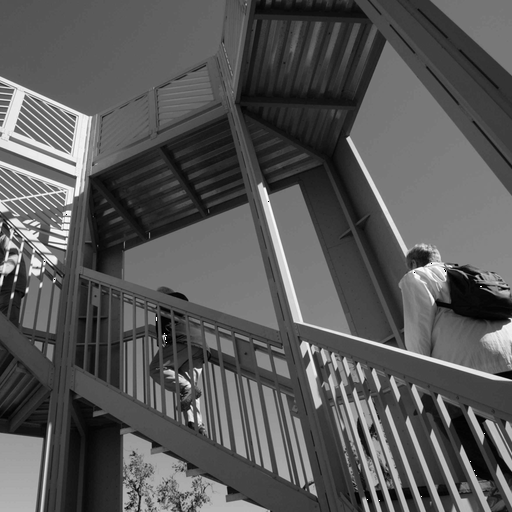
\includegraphics[width=.4\linewidth]{ascent.png}}
 \hfill
 \subfloat[Segmented region.]{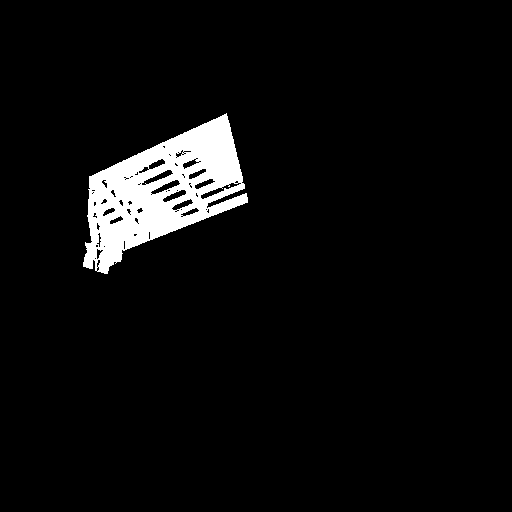
\includegraphics[width=.4\linewidth]{predicate_seg.python.png}} 
 
 \subfloat[Segmented region.]{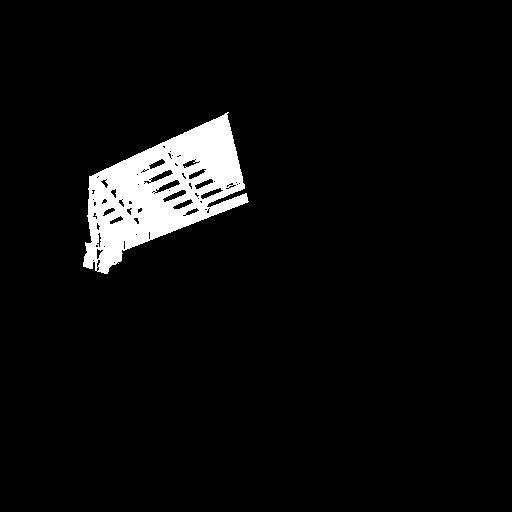
\includegraphics[width=.4\linewidth]{predicate2_seg.python.png}} 
 \hfill\subfloat[Segmented region.]{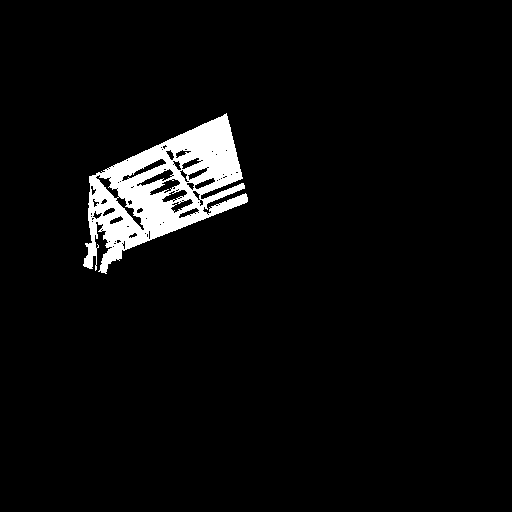
\includegraphics[width=.4\linewidth]{predicate3_seg.python.png}}%
 \label{fig:regiongrowing:python:result}%
\end{figure}
